% Provenance (never printed): see sources/outline_sources.md (Year 2: humidity variables;
% Clausius--Clapeyron applied; dry and moist adiabats; thermodynamic diagrams; convective
% instability; cloud microphysics). Definitions after the NWS glossary; skew-T lines, CAPE classes
% and the lifted index after the NWS Houston/Galveston training page; saturation data from the
% NIST WebBook (IAPWS-95) and IAPWS R14-08; the empirical formula as used by Su and others
% (2026); kappa-Koehler theory after Petters and Kreidenweis (2007); CCN numbers after Andreae
% (2009); the processes of microphysics after Morrison and others (2020). The sounding is the
% real 12 UTC sounding of Norman, Oklahoma, 16 April 2026 (IGRA2); every curve and number from
% figdata/bachelor-2/thermo.py; exercise and problem values in the Book 4 scratch calculator
% calc/ch21.py.
\chapter{Termodinámica atmosférica}\label{ch:b2:atmospheric-thermodynamics}

El 16 de abril de 2026, a las 12 UTC, un globo se elevó desde la estación meteorológica de Norman (Oklahoma), como
se elevan a esa hora, cada día, globos desde más de ochocientas estaciones. El instrumento que
llevaba transmitió por radio un perfil vertical que un predictor lee de un vistazo: aire casi saturado
cerca del suelo, una delgada tapa cálida a seiscientos metros de altura y, por encima, una temperatura que caía
deprisa a lo largo de diez kilómetros. Elevado a través de la tapa, el aire de superficie se habría encontrado
más cálido que su entorno en la mayor parte de la troposfera, con unos dos mil julios por
kilogramo para gastar en subir. En este capítulo se aprende a leer esa energía en un sondeo: cuánta
agua contiene el aire, cómo se enfría una porción que asciende antes y después de condensarse, cómo los diagramas de
los meteorólogos convierten áreas en energías y cómo llegan a formarse las gotitas de las nubes.
% ledger: data:b4-sounding, nws4:upperair, nws4:cape

\begin{recall}
\textbf{De los libros de física}: la \omterm{def:b2:atmospheric-thermodynamics:moist-air}{presión de vapor} de saturación, la humedad relativa, el punto de rocío,
el calor latente, la relación de Clausius--Clapeyron y su forma integrada; la nucleación y la
sobrefusión; el primer principio, las transformaciones adiabáticas y las capacidades caloríficas de un gas ideal.
\textbf{De los libros de química}: las presiones parciales, la ley de Raoult, la tensión superficial y la ecuación
de Kelvin. \textbf{De los volúmenes escolares}: el \omterm{def:b2:atmospheric-thermodynamics:lcl}{nivel de condensación} y su regla de
\qty{125}{m} por grado, el aire estable e inestable, el \omterm{def:b2:atmospheric-thermodynamics:microphysics}{núcleo de condensación}, los procesos de lluvia cálida
y de cristales de hielo. \textbf{Del volumen de primer año}: la atmósfera estándar, el gradiente ambiental
y el gradiente adiabático seco ($\Gamma_d = \qty{9.8}{K/km}$), la porción de aire, la temperatura
potencial, la estabilidad estática, las inversiones térmicas y la ecuación hipsométrica.
\end{recall}

En todo el capítulo: $R_d = R/M_d = \qty{287.0}{J.kg^{-1}.K^{-1}}$ para el aire seco, de masa molar
\qty{28.97}{g/mol}; $R_v = R/M_w = \qty{461.5}{J.kg^{-1}.K^{-1}}$ para el vapor de agua, de masa
molar \qty{18.0153}{g/mol}; $\varepsilon = M_w/M_d = 0.622$; $c_p = \tfrac72 R_d =
\qty{1004.5}{J.kg^{-1}.K^{-1}}$ (el volumen de primer año, con el cociente de capacidades caloríficas 1.4);
$g = \qty{9.81}{m.s^{-2}}$; y el calor latente de vaporización en el punto triple,
$L = \qty{2.501e6}{J/kg}$.
% ledger: const:R, earth:Mmol, nist4:water-mw, nasa:grc-gamma, const:gn, nist4:water-sat

\section{El aire húmedo}\label{sec:b2:atmospheric-thermodynamics:moist-air}

El aire es una mezcla de aire seco y vapor de agua, ambos próximos a gases ideales. Los libros de física
miden su agua por la humedad relativa y el punto de rocío; una porción que asciende necesita medidas
que no cambien cuando se expande.

\begin{definition}[Presión de vapor; razón de mezcla; humedad específica]\label{def:b2:atmospheric-thermodynamics:moist-air}
La \emph{presión de vapor}\index{presion de vapor@presión de vapor} $e$ del aire húmedo es la presión parcial de
su vapor de agua. Su \emph{razón de mezcla}\index{razon de mezcla@razón de mezcla} es $r = m_v/m_d$, la masa de vapor
de agua por unidad de masa de aire seco en el mismo volumen, y su \emph{humedad
específica}\index{humedad especifica@humedad específica} es $q = m_v/(m_d + m_v)$, la masa de vapor por unidad de masa de
aire húmedo. Ambas se dan habitualmente en gramos por kilogramo.
\end{definition}
% ledger: nws4:humidity

\begin{proposition}[Variables de humedad]\label{prop:b2:atmospheric-thermodynamics:humidity}
En aire húmedo a la presión total $p$ y con la \omterm{def:b2:atmospheric-thermodynamics:moist-air}{presión de vapor} $e$,
\[
  r = \frac{\varepsilon e}{p - e}, \qquad q = \frac{r}{1 + r} = \frac{\varepsilon e}{p - (1 -
  \varepsilon)e} .
\]
En la saturación, $e = e_s(T)$ y $r = r_s(T, p)$, la \omterm{def:b2:atmospheric-thermodynamics:moist-air}{razón de mezcla} de saturación. Ni $r$ ni
$q$ cambian cuando una porción se expande o se comprime sin ganar ni perder agua.
\end{proposition}

\begin{proof}
En el mismo volumen $V$ a la temperatura $T$, cada gas obedece su propia ley de los gases ideales con su
presión parcial: $m_v = eV/(R_vT)$ y $m_d = (p - e)V/(R_dT)$, así que $r = (R_d/R_v)\,e/(p - e)$,
y $R_d/R_v = M_w/M_d = \varepsilon$. Dividiendo $m_v$ por $m_d + m_v$ se obtiene $q = r/(1 + r)$.
La expansión cambia $V$, $p$ y $e$, pero no las dos masas.
\end{proof}

\begin{definition}[Temperatura virtual]\label{def:b2:atmospheric-thermodynamics:virtual}
La \emph{temperatura virtual}\index{temperatura virtual} $T_v$ del aire húmedo es la temperatura
que necesitaría el aire seco, a la misma presión, para tener la misma densidad:
\[
  T_v = T\,\frac{1 + r/\varepsilon}{1 + r} \approx T\,(1 + 0.61\,r) .
\]
\end{definition}
% ledger: nws4:virtual-theta-e

La demostración de que esta temperatura hace lo que dice cabe en una línea: la densidad del aire húmedo es
$(m_d + m_v)/V = \bigl(p - e\bigr)/(R_dT) + e/(R_vT)$, que, con $e = pr/(\varepsilon + r)$,
es igual a $p/(R_dT_v)$. El vapor de agua es más ligero que el aire seco, así que el aire húmedo es menos denso que el aire
seco a la misma temperatura y presión, como si fuera un poco más cálido.

\begin{example}[El aire de Norman]\label{ex:b2:atmospheric-thermodynamics:norman}
En el suelo, el sondeo da $p = \qty{971.1}{hPa}$, $T = \qty{19.0}{\celsius}$ y un punto de
rocío de \qty{18.5}{\celsius}. La \omterm{def:b2:atmospheric-thermodynamics:moist-air}{presión de vapor} es la \omterm{def:b2:atmospheric-thermodynamics:moist-air}{presión de vapor} de saturación en el punto
de rocío, $e = e_s(\qty{18.5}{\celsius}) = \qty{21.5}{hPa}$ (\cref{prop:b2:atmospheric-thermodynamics:es}
más abajo). Entonces $r = 0.622 \times 21.5/(971.1 - 21.5) = \qty{14.1}{g/kg}$, $q = \qty{13.9}{g/kg}$,
y $T_v - T = 0.61 \times 0.0141 \times \qty{292.15}{K} = \qty{2.5}{K}$: este aire es tan ligero como
aire seco dos grados y medio más cálido.
\end{example}
% ledger: data:b4-sounding

\section{La presión de vapor de saturación}\label{sec:b2:atmospheric-thermodynamics:saturation}

Sobre una superficie plana de agua pura, la \omterm{def:b2:atmospheric-thermodynamics:moist-air}{presión de vapor} en equilibrio solo depende de la
temperatura. Los libros de física deducen su ley, la relación de Clausius--Clapeyron, y la integran
con un calor latente constante; para el vapor de agua, $M L/R = L/R_v$.

\begin{proposition}[Presión de vapor de saturación]\label{prop:b2:atmospheric-thermodynamics:es}
Con el calor latente $L$ constante, la \omterm{def:b2:atmospheric-thermodynamics:moist-air}{presión de vapor} de saturación sobre el agua es
\[
  e_s(T) = e_t \exp\!\Bigl[\frac{L}{R_v}\Bigl(\frac{1}{T_t} - \frac{1}{T}\Bigr)\Bigr],
  \qquad e_t = \qty{6.117}{hPa}, \quad T_t = \qty{273.16}{K}, \quad \frac{L}{R_v} =
  \qty{5419}{K},
\]
donde $(T_t, e_t)$ es el punto triple del agua.
\end{proposition}
% ledger: iapws4:sublimation, nist4:water-sat

\begin{corollary}[Siete por ciento por kelvin]\label{cor:b2:atmospheric-thermodynamics:seven}
La tasa relativa de aumento de la \omterm{def:b2:atmospheric-thermodynamics:moist-air}{presión de vapor} de saturación es
$\mathrm{d}\ln e_s/\mathrm{d}T = L/(R_v T^2)$: un \qty{7.3}{\percent} por kelvin a
\qty{0}{\celsius}, un \qty{6.3}{\percent} a \qty{20}{\celsius} y un \qty{5.9}{\percent} a
\qty{30}{\celsius}.
\end{corollary}

El calor latente constante es el único defecto de la fórmula: el calor latente baja de
\qty{2500.9}{kJ/kg} en el punto triple a \qty{2453.5}{kJ/kg} a \qty{20}{\celsius}, de modo que la
fórmula se adelanta a los valores medidos a medida que sube la temperatura, en un \qty{1.2}{\percent} a
\qty{20}{\celsius} y un \qty{2.5}{\percent} a \qty{30}{\celsius} (figura de abajo). Una fórmula
empírica ajustada a las medidas, $e_s = \qty{6.112}{hPa} \times \exp[17.67\,t/(t + 243.5)]$ con
$t$ en grados Celsius, se mantiene a unas pocas milésimas; los productos de datos la usan, pero la
proposición es la que puede derivarse y entenderse, y este capítulo se queda con ella.
% ledger: nist4:water-sat, su26:svp

Por debajo de \qty{0}{\celsius}, el agua puede seguir líquida en las nubes, en sobrefusión, y existen dos presiones de vapor
de saturación: sobre el agua líquida y sobre el hielo. La segunda es menor, porque el calor latente
de sublimación supera al de vaporización en el calor latente de fusión. El aire saturado
respecto de las gotitas sobrefundidas está sobresaturado respecto del hielo, en un \qty{10}{\percent} a
\qty{-10}{\celsius} y un \qty{22}{\percent} a \qty{-20}{\celsius}: la última sección vuelve sobre
esa diferencia.
% ledger: iapws4:sublimation, su26:svp

\begin{omfigure}
\centering
% figdata/bachelor-2/thermo.py parts es, nist
\begin{tikzpicture}
\begin{groupplot}[group style={group size=2 by 1, horizontal sep=1.9cm},
  width=0.44\linewidth, height=5.4cm, tick label style={font=\scriptsize},
  label style={font=\small}]
\nextgroupplot[xmin=-40, xmax=40, ymin=0, ymax=80, xlabel={temperatura (\unit{\celsius})},
  ylabel={presión de vapor de saturación (\unit{hPa})}, legend pos=north west,
  legend style={font=\scriptsize, draw=none, fill=none}, legend cell align=left]
\addplot[ocBlue, thick] table[x=T_C, y=cc] {figdata/out/bachelor-2-thermo-es.dat};
\addlegendentry{proposición}
\addplot[black, densely dashed] table[x=T_C, y=emp] {figdata/out/bachelor-2-thermo-es.dat};
\addlegendentry{fórmula empírica}
\addplot[only marks, mark=*, mark size=1.4pt, ocRed] table[x=T_C, y=es_hPa]
  {figdata/out/bachelor-2-thermo-nist.dat};
\addlegendentry{medida (IAPWS-95)}
\nextgroupplot[xmin=-40, xmax=0, ymin=1, ymax=1.5, xlabel={temperatura (\unit{\celsius})},
  ylabel={$e_s(\text{agua})/e_s(\text{hielo})$}]
\addplot[omMeth, thick, unbounded coords=discard] table[x=T_C, y=wi]
  {figdata/out/bachelor-2-thermo-es.dat};
\draw[black!40, densely dotted] (axis cs:-10,1) -- (axis cs:-10,1.1035) -- (axis cs:-40,1.1035);
\node[font=\scriptsize, anchor=south west] at (axis cs:-10,1.1035) {1.10};
\draw[black!40, densely dotted] (axis cs:-20,1) -- (axis cs:-20,1.218) -- (axis cs:-40,1.218);
\node[font=\scriptsize, anchor=south west] at (axis cs:-20,1.218) {1.22};
\end{groupplot}
\end{tikzpicture}
\par\smallskip{\small Izquierda: la \omterm{def:b2:atmospheric-thermodynamics:moist-air}{presión de vapor} de saturación sobre el agua según la
\cref{prop:b2:atmospheric-thermodynamics:es}, según la fórmula empírica y medida. Derecha: el
cociente de las presiones de vapor de saturación sobre el agua sobrefundida (fórmula empírica) y sobre el hielo
(ecuación de sublimación de la IAPWS).}
\end{omfigure}
% ledger: nist4:water-sat, iapws4:sublimation, su26:svp

\section{El aire húmedo que asciende}\label{sec:b2:atmospheric-thermodynamics:ascent}

Una porción que asciende sin intercambiar calor se enfría según el gradiente adiabático seco, conserva su
temperatura potencial y, si no se condensa, conserva su \omterm{def:b2:atmospheric-thermodynamics:moist-air}{razón de mezcla}. Su \omterm{def:b2:atmospheric-thermodynamics:moist-air}{presión de vapor}
$e = pr/(\varepsilon + r)$ disminuye con la presión, pero su \omterm{def:b2:atmospheric-thermodynamics:moist-air}{presión de vapor} de saturación disminuye
más deprisa, con su temperatura. Las dos se encuentran en un nivel que los volúmenes escolares hallaban con una regla.

\begin{definition}[Nivel de condensación por ascenso]\label{def:b2:atmospheric-thermodynamics:lcl}
El \emph{nivel de condensación por ascenso}\index{nivel de condensacion por ascenso@nivel de condensación por ascenso} (NCA) de una porción es el
nivel en el que se satura cuando se eleva adiabáticamente en seco. Es el
\emph{nivel de condensación}\index{nivel de condensacion@nivel de condensación} de los volúmenes escolares, la altura de las
bases planas de las nubes que se forman por ascenso.
\end{definition}
% ledger: nws4:lcl

\begin{proposition}[Altura del nivel de condensación por ascenso]\label{prop:b2:atmospheric-thermodynamics:lcl}
Una porción a la temperatura $T$ con el punto de rocío $T_d$ alcanza la saturación aproximadamente a
\[
  z_{\text{NCA}} \approx \frac{T - T_d}{\Gamma_d - \Gamma_{\text{roc}}}, \qquad
  \Gamma_{\text{roc}} = \frac{g R_v T_d^2}{L R_d T} \approx \qty{1.8}{K/km},
\]
por encima de su nivel de partida: unos \qty{125}{m} por cada grado de depresión del punto de rocío.
\end{proposition}

\begin{proof}
La temperatura de la porción baja según $\Gamma_d$. Su punto de rocío es la temperatura a la que su
\omterm{def:b2:atmospheric-thermodynamics:moist-air}{presión de vapor} $e$ sería de saturación; con $r$ constante, $e$ es proporcional a $p$, así que
$\mathrm{d}\ln e = \mathrm{d}\ln p = -g\,\mathrm{d}z/(R_dT)$ por el equilibrio hidrostático. Por la
\cref{prop:b2:atmospheric-thermodynamics:es}, $\mathrm{d}\ln e = L\,\mathrm{d}T_d/(R_vT_d^2)$.
Por tanto $\mathrm{d}T_d/\mathrm{d}z = -gR_vT_d^2/(LR_dT) = -\Gamma_{\text{roc}}$: el punto de rocío también baja,
pero más despacio. La diferencia $T - T_d$ se cierra al ritmo $\Gamma_d - \Gamma_{\text{roc}}$. Con
$T \approx T_d \approx \qty{288}{K}$, $\Gamma_{\text{roc}} = \qty{1.8}{K/km}$, y $1/(9.8 - 1.8)$
kilómetros por kelvin son \qty{125}{m}.
\end{proof}

En Norman la depresión del punto de rocío era de \qty{0.5}{K}: el aire de superficie se habría condensado tras
\qty{63}{m} de ascenso, a \qty{964}{hPa}. El cálculo completo, que sigue la adiabática seca y
la \omterm{def:b2:atmospheric-thermodynamics:moist-air}{razón de mezcla} de saturación sin linealizar, da \qty{64}{m}.
% ledger: data:b4-sounding

Por encima del NCA la porción se condensa a medida que sube. La condensación libera calor latente, y la porción
se enfría más despacio.

\begin{definition}[Gradiente adiabático saturado; adiabática húmeda]\label{def:b2:atmospheric-thermodynamics:moist-adiabat}
El \emph{gradiente adiabático saturado}\index{gradiente adiabatico saturado@gradiente adiabático saturado} $\Gamma_s$ es
el ritmo al que baja la temperatura de una porción saturada cuando asciende, mientras su vapor se condensa
para mantenerla saturada. La curva que sigue en un diagrama de temperatura frente a presión es una
\emph{adiabática húmeda}\index{adiabatica humeda@adiabática húmeda}. Cuando se supone que el agua condensada cae
de inmediato, el ascenso se llama pseudoadiabático.
\end{definition}
% ledger: nws4:malr

\begin{proposition}[Gradiente adiabático saturado]\label{prop:b2:atmospheric-thermodynamics:gamma-s}
Para un ascenso pseudoadiabático, con $r_s = r_s(T, p)$,
\[
  \Gamma_s = g\,\frac{1 + \dfrac{L r_s}{R_d T}}{c_p + \dfrac{L^2 r_s}{R_v T^2}} .
\]
Tiende a $\Gamma_d = g/c_p$ cuando $r_s$ tiende a cero, y es menor en los demás casos.
\end{proposition}

\begin{proof}
Por unidad de masa de aire seco, el primer principio para una porción que recibe el calor latente del vapor
que condensa, $-L\,\mathrm{d}r_s$, se escribe $c_p\,\mathrm{d}T - (R_dT/p)\,\mathrm{d}p = -L\,
\mathrm{d}r_s$; con el equilibrio hidrostático $(R_dT/p)\,\mathrm{d}p = -g\,\mathrm{d}z$, queda
$c_p\,\mathrm{d}T + g\,\mathrm{d}z + L\,\mathrm{d}r_s = 0$. Con $r_s \approx \varepsilon e_s/p$,
$\mathrm{d}r_s = r_s\,(\mathrm{d}\ln e_s - \mathrm{d}\ln p) = r_s\bigl(L\,\mathrm{d}T/(R_vT^2) +
g\,\mathrm{d}z/(R_dT)\bigr)$. Sustituyendo y agrupando los términos en $\mathrm{d}T$ y en
$\mathrm{d}z$ se obtiene $-\mathrm{d}T/\mathrm{d}z = \Gamma_s$.
\end{proof}

El gradiente depende de cuánta agua haya para condensar. A \qty{1000}{hPa} vale
\qty{6.5}{K/km} a \qty{0}{\celsius}, \qty{5.2}{K/km} a \qty{10}{\celsius}, \qty{4.2}{K/km} a
\qty{20}{\celsius} y \qty{3.4}{K/km} a \qty{30}{\celsius}; en lo alto de la troposfera, a
\qty{200}{hPa} y \qty{-60}{\celsius}, vuelve a \qty{9.6}{K/km}, casi el gradiente seco. Una
\omterm{def:b2:atmospheric-thermodynamics:moist-adiabat}{adiabática húmeda} es, pues, empinada cerca del suelo cálido y se curva hacia las adiabáticas secas en altura.
% ledger: nws4:malr

\begin{definition}[Temperatura potencial equivalente]\label{def:b2:atmospheric-thermodynamics:theta-e}
La \emph{temperatura potencial equivalente}\index{temperatura potencial equivalente} $\theta_e$ de
una porción es la temperatura que tendría si se elevara hasta que todo su vapor se hubiera condensado
y precipitado, y después se bajara adiabáticamente en seco hasta \qty{1000}{hPa}. Una buena aproximación es
\[
  \theta_e \approx \theta \exp\!\Bigl(\frac{L r}{c_p T_{\text{NCA}}}\Bigr),
\]
con $\theta$ la temperatura potencial y $T_{\text{NCA}}$ la temperatura en el \omterm{def:b2:atmospheric-thermodynamics:lcl}{nivel de condensación
por ascenso} de la porción.
\end{definition}
% ledger: nws4:virtual-theta-e

La temperatura potencial solo se conserva en el ascenso seco; $\theta_e$ se conserva, con esta
aproximación, tanto en el ascenso seco como en el saturado, porque el calor que cuenta como ya liberado
es exactamente el calor que libera la condensación. Etiqueta una \omterm{def:b2:atmospheric-thermodynamics:moist-adiabat}{adiabática húmeda} como $\theta$ etiqueta una seca.
El aire de superficie de Norman tiene $\theta = 292.15 \times (1000/971.1)^{2/7} = \qty{294.6}{K}$ y
$\theta_e = 294.6 \exp[2.501 \times 10^6 \times 0.0141/(1004.5 \times 291.5)] = \qty{332}{K}$.
% ledger: data:b4-sounding

\section{Diagramas termodinámicos}\label{sec:b2:atmospheric-thermodynamics:diagrams}

\begin{definition}[Sondeo atmosférico]\label{def:b2:atmospheric-thermodynamics:sounding}
Un \emph{sondeo atmosférico}\index{sondeo atmosferico@sondeo atmosférico} es un perfil vertical de la
presión, la temperatura, la humedad y el viento de la atmósfera sobre un lugar, medido por un
instrumento llevado hacia arriba, normalmente una radiosonda colgada de un globo.
\end{definition}
% ledger: nws:radiosonde, nws4:upperair

Un sondeo no es del todo vertical, porque el globo deriva con el viento, ni del todo
instantáneo, porque tarda varios minutos en llegar a la troposfera alta; y la red principal
solo lanza dos veces al día. Sus cifras se vuelven útiles una vez dibujadas en un gráfico
donde una porción que asciende puede seguirse con una regla.
% ledger: hgx:skewt-lines

\begin{definition}[Diagrama termodinámico; diagrama skew-T log-p; tefigrama]\label{def:b2:atmospheric-thermodynamics:diagram}
Un \emph{diagrama termodinámico}\index{diagrama termodinamico@diagrama termodinámico} es un gráfico cuyas coordenadas son
funciones de la presión y la temperatura, en el que van impresas isobaras, isotermas, adiabáticas secas, \omterm{def:b2:atmospheric-thermodynamics:moist-adiabat}{adiabáticas
húmedas} y líneas de \omterm{def:b2:atmospheric-thermodynamics:moist-air}{razón de mezcla} de saturación constante, y en el que un sondeo se
representa con dos curvas, su temperatura y su punto de rocío. En un \emph{diagrama skew-T
log-p}\index{diagrama skew-T log-p} la coordenada vertical es $-\ln p$ y la horizontal es
$T + k\ln(p_0/p)$, de modo que las isobaras son horizontales y las isotermas son rectas inclinadas hacia arriba
a la derecha. Un \emph{tefigrama}\index{tefigrama} usa como coordenadas la temperatura y la entropía por unidad
de masa $c_p\ln\theta$, de modo que las isotermas y las adiabáticas secas son rectas
perpendiculares.
\end{definition}
% ledger: hgx:skewt-lines

\begin{proposition}[Las áreas son energías]\label{prop:b2:atmospheric-thermodynamics:areas}
En un \omterm{def:b2:atmospheric-thermodynamics:diagram}{diagrama skew-T log-p}, el área encerrada entre dos curvas $T_1(p)$ y $T_2(p)$ sobre las
presiones $p_b > p_a$ es proporcional a $\int_{p_a}^{p_b} R_d\,(T_1 - T_2)\,\mathrm{d}\ln p$,
la energía por unidad de masa que la \cref{prop:b2:atmospheric-thermodynamics:buoyancy} de más abajo da a
una porción que sigue $T_1$ a través de un entorno $T_2$.
\end{proposition}

\begin{proof}
Tómese $Y = \ln(p_0/p)$ y $X = T + kY$. El jacobiano de $(T, Y) \mapsto (X, Y)$ vale 1, así que las áreas en
el plano $(X, Y)$ son iguales a las áreas en el plano $(T, Y)$, donde el área entre dos curvas es
$\int (T_1 - T_2)\,\mathrm{d}Y = \int (T_1 - T_2)\,\mathrm{d}\ln p$ tomada de $p_a$ a $p_b$
con el signo fijado. Multiplicando por $R_d$ y por la escala del gráfico se obtiene la energía.
\end{proof}

\begin{method}[Elevar una porción en un diagrama]\label{met:b2:atmospheric-thermodynamics:lift}
\begin{enumerate}
  \item Represéntense la temperatura y el punto de rocío del sondeo frente a la presión.
  \item Desde la temperatura de la porción, sígase la adiabática seca hacia arriba; desde su punto de rocío, sígase
        la línea de \omterm{def:b2:atmospheric-thermodynamics:moist-air}{razón de mezcla} de saturación. Donde se cortan está el NCA.
  \item Desde el NCA, sígase la \omterm{def:b2:atmospheric-thermodynamics:moist-adiabat}{adiabática húmeda} hacia arriba.
  \item Donde la curva de la porción queda a la derecha de la temperatura del sondeo, la porción es
        más cálida que su entorno; los niveles donde se cruzan las dos curvas son los niveles de la
        \cref{def:b2:atmospheric-thermodynamics:parcel-levels} de más abajo.
\end{enumerate}
\end{method}
% ledger: hgx:skewt-lines


\section{Estabilidad y energía convectiva}\label{sec:b2:atmospheric-thermodynamics:stability}

El volumen de primer año comparaba el gradiente $\Gamma$ de una capa con $\Gamma_d$. Una porción saturada
se enfría en cambio según $\Gamma_s$, y aparece un tercer caso entre los dos gradientes.

\begin{definition}[Inestabilidad condicional]\label{def:b2:atmospheric-thermodynamics:instability}
Una capa cuyo gradiente está comprendido entre el \omterm{def:b2:atmospheric-thermodynamics:moist-adiabat}{gradiente adiabático saturado} y el seco,
$\Gamma_s < \Gamma < \Gamma_d$, está en
\emph{inestabilidad condicional}\index{inestabilidad condicional}: es estable para las porciones no saturadas e inestable para las saturadas.
\end{definition}
% ledger: nws4:malr

En Norman la temperatura bajó \qty{37.0}{K} entre \qty{850}{hPa} (\qty{1489}{m}) y
\qty{500}{hPa} (\qty{5725}{m}), a \qty{8.7}{K/km}: \omterm{def:b2:atmospheric-thermodynamics:instability}{inestabilidad condicional} a lo largo de cuatro kilómetros.
Que la inestabilidad se libere depende de dónde una porción procedente de abajo se satura y
luego se vuelve más cálida que su entorno.
% ledger: data:b4-sounding

\begin{definition}[Nivel de convección libre; nivel de equilibrio]\label{def:b2:atmospheric-thermodynamics:parcel-levels}
El \emph{nivel de convección libre}\index{nivel de conveccion libre@nivel de convección libre} (NCL) de una porción elevada es
el nivel por encima del cual, saturada, se vuelve más cálida que su entorno y asciende libremente. El
\emph{nivel de equilibrio}\index{nivel de equilibrio} (NE) es el nivel por encima del NCL en el que su
temperatura vuelve a igualar la de su entorno.
\end{definition}
% ledger: nws4:lfc-el

\begin{omfigure}
\centering
% figdata/bachelor-2/thermo.py parts iso, dry, moist, mix, env, dew, parcel, cape, cin, marks
\begin{tikzpicture}
\begin{axis}[width=0.86\linewidth, height=10.6cm, ymode=log, y dir=reverse, ymin=100,
  ymax=1050, xmin=-42, xmax=44, clip=true,
  ytick={100,200,300,400,500,700,850,1000}, yticklabels={100,200,300,400,500,700,850,1000},
  minor ytick={}, xtick={-41.464,-31.464,-21.464,-11.464,-1.464,8.536,18.536,28.536,38.536},
  xticklabels={$-40$,$-30$,$-20$,$-10$,0,10,20,30,40}, tick label style={font=\scriptsize},
  xlabel={temperatura (\unit{\celsius}), leída a lo largo de las isotermas inclinadas},
  ylabel={presión (\unit{hPa})}, label style={font=\small},
  legend style={font=\scriptsize, at={(0.985,0.985)}, anchor=north east, fill=white,
  fill opacity=0.9, text opacity=1, draw=black!30}, legend cell align=left]
\addplot[fill=ocRed, fill opacity=0.28, draw=none, forget plot] table[x=x, y=p]
  {figdata/out/bachelor-2-thermo-cape.dat};
\addplot[fill=ocBlue, fill opacity=0.28, draw=none, forget plot] table[x=x, y=p]
  {figdata/out/bachelor-2-thermo-cin.dat};
\addplot[black!22, very thin, forget plot] table[x=x, y=p] {figdata/out/bachelor-2-thermo-iso.dat};
\addplot[orange!70!black, very thin, opacity=0.55] table[x=x, y=p]
  {figdata/out/bachelor-2-thermo-dry.dat};
\addlegendentry{adiabáticas secas}
\addplot[omMeth, very thin, densely dashed, opacity=0.7] table[x=x, y=p]
  {figdata/out/bachelor-2-thermo-moist.dat};
\addlegendentry{adiabáticas húmedas}
\addplot[ocBlue, thin, dotted] table[x=x, y=p]
  {figdata/out/bachelor-2-thermo-mix.dat};
\addlegendentry{razón de mezcla de saturación}
\addplot[ocRed, thick] table[x=x, y=p] {figdata/out/bachelor-2-thermo-env.dat};
\addlegendentry{temperatura}
\addplot[omMeth!70!black, thick] table[x=x, y=p] {figdata/out/bachelor-2-thermo-dew.dat};
\addlegendentry{punto de rocío}
\addplot[black, thick, dashed] table[x=x, y=p] {figdata/out/bachelor-2-thermo-parcel.dat};
\addlegendentry{porción de superficie}
\foreach \r/\x in {1/-7.948, 2/0.283, 4/9.053, 8/18.396, 16/28.323} {
  \edef\tmp{\noexpand\node[font=\noexpand\tiny, ocBlue, anchor=south] at (axis cs:\x,600) {\r};}\tmp
}
\addplot[only marks, mark=*, mark size=1.6pt, black, forget plot] table[x=x, y=p]
  {figdata/out/bachelor-2-thermo-marks.dat};
\node[font=\scriptsize, anchor=west] at (axis cs:20.5,963.9) {NCA};
\node[font=\scriptsize, anchor=west] at (axis cs:18.2,732.5) {NCL};
\node[font=\scriptsize, anchor=east] at (axis cs:-9.6,235.6) {NE};
\node[font=\scriptsize, ocRed!70!black] at (axis cs:2,420) {CAPE};
\node[font=\scriptsize, ocBlue!70!black, anchor=west] at (axis cs:27,860) {CIN};
\end{axis}
\end{tikzpicture}
\par\smallskip{\small El sondeo de las 12 UTC de Norman (Oklahoma) del 16 de abril de 2026, en un \omterm{def:b2:atmospheric-thermodynamics:diagram}{diagrama
skew-T log-p}, con la porción de superficie elevada a lo largo de su adiabática seca hasta el NCA y de su \omterm{def:b2:atmospheric-thermodynamics:moist-adiabat}{adiabática
húmeda} por encima. En rojo, el área positiva (CAPE); en azul, el área negativa por debajo del NCL (CIN), ambas
calculadas con la temperatura. Razones de mezcla de saturación en gramos por kilogramo, rotuladas a
\qty{600}{hPa}.}
\end{omfigure}
% ledger: data:b4-sounding, hgx:skewt-lines

\begin{definition}[Energía potencial convectiva disponible; inhibición convectiva]\label{def:b2:atmospheric-thermodynamics:cape}
La \emph{energía potencial convectiva disponible}\index{energia potencial convectiva disponible@energía potencial convectiva disponible}
(CAPE) de una porción es el trabajo de la fuerza de flotación sobre la unidad de masa de esta entre su NCL y su
NE,
\[
  \text{CAPE} = \int_{z_{\text{NCL}}}^{z_{\text{NE}}} g\,\frac{T_{v,\text{porción}} -
  T_{v,\text{ent}}}{T_{v,\text{ent}}}\,\mathrm{d}z ,
\]
y su \emph{inhibición convectiva}\index{inhibicion convectiva@inhibición convectiva} (CIN) es la misma integral,
negativa, desde su nivel de partida hasta su NCL.
\end{definition}
% ledger: nws4:cape, nws4:cin

\begin{proposition}[La flotación en un diagrama; la velocidad de la porción]\label{prop:b2:atmospheric-thermodynamics:buoyancy}
\begin{enumerate}
  \item En términos de presión, $\text{CAPE} = R_d \int_{p_{\text{NE}}}^{p_{\text{NCL}}}
        (T_{v,\text{porción}} - T_{v,\text{ent}})\,\mathrm{d}\ln p$: en un \omterm{def:b2:atmospheric-thermodynamics:diagram}{diagrama skew-T log-p} es
        proporcional al área entre la curva de la porción y el sondeo.
  \item Una porción que sale del NCL en reposo y conserva todo el trabajo de su flotación llega al
        NE con la velocidad vertical $w_{\max} = \sqrt{2\,\text{CAPE}}$.
\end{enumerate}
\end{proposition}

\begin{proof}
1. La porción y su entorno comparten la presión, así que el cociente de densidades es el cociente de las
\omterm{def:b2:atmospheric-thermodynamics:virtual}{temperaturas virtuales} y la fuerza de flotación por unidad de masa es
$g(T_{v,\text{porción}} - T_{v,\text{ent}})/T_{v,\text{ent}}$. El entorno es hidrostático:
$\mathrm{d}z = -R_dT_{v,\text{ent}}\,\mathrm{d}\ln p/g$. Al sustituir se simplifican $g$ y
$T_{v,\text{ent}}$; el área se sigue de la \cref{prop:b2:atmospheric-thermodynamics:areas}.
2. Con $b$ la fuerza de flotación por unidad de masa, $\mathrm{d}w/\mathrm{d}t = b$ y $w = \mathrm{d}z/
\mathrm{d}t$ dan $w\,\mathrm{d}w = b\,\mathrm{d}z$; integrando desde el NCL, donde $w = 0$, hasta
el NE se obtiene $w^2/2 = \text{CAPE}$.
\end{proof}

\begin{example}[La energía del sondeo de Norman]\label{ex:b2:atmospheric-thermodynamics:cape}
Elévese el aire de superficie del \cref{ex:b2:atmospheric-thermodynamics:norman}. Se satura a
\qty{964}{hPa}, \qty{64}{m} más arriba, y sigue una \omterm{def:b2:atmospheric-thermodynamics:moist-adiabat}{adiabática húmeda}. Por debajo de \qty{900}{hPa} el sondeo está
él mismo casi saturado y la porción se mantiene unas décimas de grado más fría que su
entorno; luego llega la inversión entre \qty{908}{hPa} y \qty{889}{hPa}, donde la
temperatura sube \qty{4.1}{K} en \qty{178}{m} y la porción se encuentra \qty{5}{K} demasiado
fría. Solo se vuelve más cálida que su entorno a \qty{732}{hPa}, \qty{2.4}{km} sobre el
suelo, su NCL, y sigue más cálida hasta su NE a \qty{236}{hPa}, \qty{10.9}{km} sobre el nivel del mar,
justo por debajo de la tropopausa que el sondeo señala a \qty{235}{hPa}. Sobre una malla fina de presiones, las
áreas de la figura skew-T dan CAPE $= \qty{2100}{J/kg}$ y CIN $= \qty{-200}{J/kg}$ con la
temperatura, y \qty{2230}{J/kg} y \qty{-130}{J/kg} con la \omterm{def:b2:atmospheric-thermodynamics:virtual}{temperatura virtual}: la humedad
de la porción añade su propia flotación. La teoría de la porción da $w_{\max} = \sqrt{2 \times 2100} =
\qty{65}{m/s}$.
\end{example}
% ledger: data:b4-sounding

Las tablas de los predictores llaman positiva a una CAPE de hasta \qty{1500}{J/kg}, grande a una de entre 1500 y
\qty{2500}{J/kg} y extrema a una de más de \qty{2500}{J/kg}; los valores de más de \qty{1000}{J/kg} son frecuentes en los entornos de tormenta,
y unos pocos superan \qty{5000}{J/kg}. La CAPE es máxima en la estación cálida, sobre todo a finales de
la primavera. El índice de levantamiento, la temperatura del sondeo a \qty{500}{hPa} menos la de la porción
elevada, resume la misma información en un solo número: en Norman, $-18.4 - (-8.9) = \qty{-9.5}{K}$,
en la clase de $-8$ a $-10$ que las tablas de los predictores llaman inestabilidad extrema. Ninguno de
estos valores es un umbral por encima del cual las tormentas deban formarse.
% ledger: hgx:cape, nws4:cape, nws4:lifted-index

La CIN es el precio de la entrada. La tapa cálida impedía que el aire de superficie subiera por sí solo: una
porción tendría que ser empujada a través de ella, por un frente o por el lento ascenso del aire que precede
a una perturbación en altura, o calentada desde abajo por el sol de la tarde hasta ser flotante en todo el recorrido.
Y la velocidad $w_{\max}$ es una cota superior: una corriente ascendente real transporta su agua condensada, que
la lastra, y se mezcla con el aire más seco que la rodea, que la enfría por evaporación. El
\omterm{def:b2:atmospheric-thermodynamics:parcel-levels}{nivel de equilibrio} sigue siendo una buena guía de dónde las cimas de la tormenta se extienden en un yunque.
% ledger: nws4:cin, hgx:cape, nws4:lfc-el

\begin{omfigure}
\centering
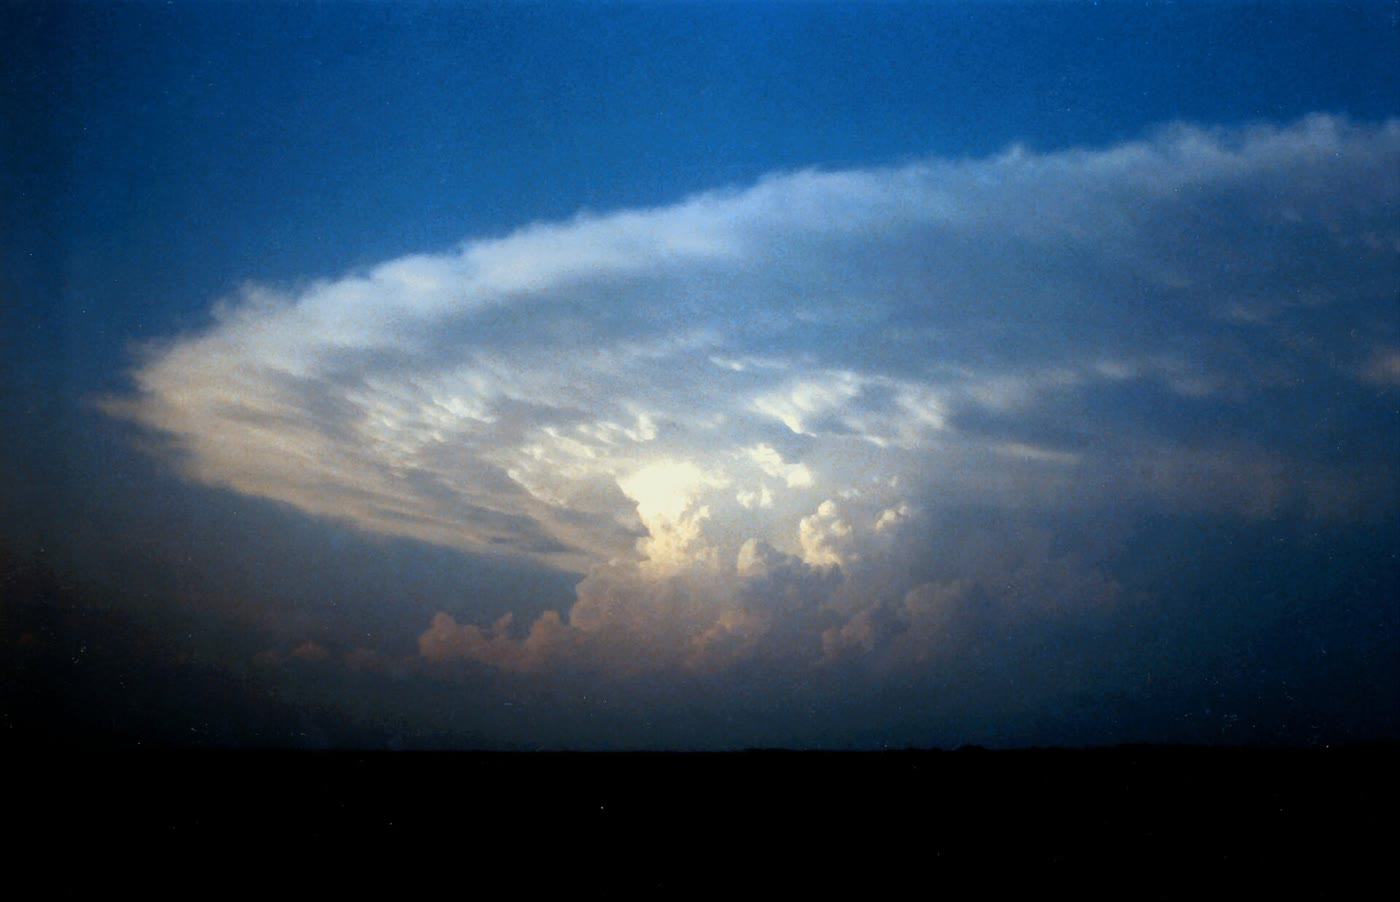
\includegraphics[width=0.6\linewidth]{images/book4/b2-21-supercell-anvil.jpg}
\par\smallskip{\small Una tormenta sobre Nebraska, el 20 de abril de 1985: su corriente ascendente se extiende en
un yunque donde alcanza su \omterm{def:b2:atmospheric-thermodynamics:parcel-levels}{nivel de equilibrio}, cerca de la tropopausa. (Stephen Corfidi,
NOAA/NWS, dominio público, a través de Wikimedia Commons.)}
\end{omfigure}
% ledger: nws4:lfc-el

\section{Microfísica de nubes}\label{sec:b2:atmospheric-thermodynamics:microphysics}

Una porción en su NCA está saturada respecto de una superficie de agua plana. Una gotita no es plana: los libros
de física muestran que una fase nueva no aparece en el equilibrio, sino solo por nucleación, y los
libros de química que la \omterm{def:b2:atmospheric-thermodynamics:moist-air}{presión de vapor} sobre una superficie curva supera a la de una superficie plana
(la ecuación de Kelvin). Con la constante $A$ de la \cref{prop:b2:atmospheric-thermodynamics:kohler}
de más abajo, una gotita de agua pura de \qty{2}{nm} de diámetro solo está en equilibrio con la razón de saturación
$\exp(2.1/2) = 2.9$, una \omterm{def:b2:atmospheric-thermodynamics:microphysics}{sobresaturación} del \qty{190}{\percent}, muy por encima de las fracciones de uno por
ciento a las que se activan las partículas: las gotitas se forman sobre partículas.

\begin{definition}[Sobresaturación; núcleo de condensación de nubes]\label{def:b2:atmospheric-thermodynamics:microphysics}
La \emph{sobresaturación}\index{sobresaturacion@sobresaturación} del aire es $s = e/e_s - 1$, el exceso de su
\omterm{def:b2:atmospheric-thermodynamics:moist-air}{presión de vapor} sobre la \omterm{def:b2:atmospheric-thermodynamics:moist-air}{presión de vapor} de saturación sobre una superficie plana de agua pura, dada
habitualmente en tanto por ciento. Un \emph{núcleo de condensación de nubes}\index{nucleo de condensacion de nubes@núcleo de condensación de nubes} (CCN)
es una partícula de aerosol sobre la que se forma una gotita de nube a las pequeñas sobresaturaciones de las nubes.
Es el \emph{núcleo de condensación}\index{nucleo de condensacion@núcleo de condensación} de los volúmenes escolares.
\end{definition}
% ledger: nws4:ccn-bergeron, pk07:kohler, morrison20:processes

\begin{proposition}[Curva de Köhler]\label{prop:b2:atmospheric-thermodynamics:kohler}
\index{curva de Kohler@curva de Köhler}
Una gotita de disolución de diámetro $D$ crecida sobre una partícula seca de diámetro $D_d$ e higroscopicidad
$\kappa$ está en equilibrio con la razón de saturación
\[
  S(D) = \frac{D^3 - D_d^3}{D^3 - D_d^3(1 - \kappa)}\,\exp\Bigl(\frac{A}{D}\Bigr), \qquad
  A = \frac{4\sigma M_w}{R T\rho_w},
\]
con $\sigma$ la tensión superficial y $\rho_w$ la densidad del agua (se admite). La curva $S(D)$
es la \emph{\omterm{prop:b2:atmospheric-thermodynamics:kohler}{curva de Köhler}}. Para $D \gg D_d$,
\[
  s = S - 1 \approx \frac{A}{D} - \frac{\kappa D_d^3}{D^3},
\]
que es máxima en el diámetro y la \omterm{def:b2:atmospheric-thermodynamics:microphysics}{sobresaturación} críticos
\[
  D_c = \sqrt{\frac{3\kappa D_d^3}{A}}, \qquad s_c = \sqrt{\frac{4A^3}{27\,\kappa D_d^3}} .
\]
\end{proposition}
% ledger: pk07:kohler

\begin{proof}[Demostración de la aproximación]
La exponencial es el factor de Kelvin; la fracción es la actividad del agua, una versión de la ley de
Raoult en la que $\kappa$ mide cuánta agua fija la materia disuelta. Para $D \gg D_d$ y
$A \ll D$, $\exp(A/D) \approx 1 + A/D$ y la fracción es $1 - \kappa D_d^3/D^3$ a primer
orden; el producto, a primer orden, es $1 + A/D - \kappa D_d^3/D^3$. Anulando la derivada
$-A/D^2 + 3\kappa D_d^3/D^4$ se obtiene $D_c^2 = 3\kappa D_d^3/A$, y entonces $s_c = A/D_c -
A/(3D_c) = 2A/(3D_c)$, que es la fórmula.
\end{proof}

Con $\sigma = \qty{0.072}{J/m^2}$ a \qty{298.15}{K}, $A = \qty{2.1}{nm}$. El sulfato de amonio tiene
$\kappa = 0.61$; el cloruro de sodio es aún más higroscópico ($\kappa = 1.28$), y las partículas atmosféricas están en su mayoría entre 0.1 y 0.9.
Una partícula seca de \qty{50}{nm} de sulfato de amonio tiene $D_c = \qty{0.33}{\micro m}$ y $s_c =
\qty{0.42}{\percent}$; una de \qty{100}{nm}, \qty{0.93}{\micro m} y \qty{0.15}{\percent}. La
aproximación difiere del máximo exacto en menos de un \qty{1}{\percent}.
% ledger: pk07:kohler, pk07:kappa

\begin{omfigure}
\centering
% figdata/bachelor-2/thermo.py part kohler
\begin{tikzpicture}
\begin{semilogxaxis}[width=0.72\linewidth, height=5.6cm, xmin=0.03, xmax=10, ymin=-0.4,
  ymax=1.1, xlabel={diámetro de la gotita $D$ (\unit{\micro m})}, ylabel={sobresaturación $s$
  (\unit{\percent})}, tick label style={font=\scriptsize}, label style={font=\small},
  log ticks with fixed point, legend style={font=\scriptsize, draw=none, fill=none},
  legend pos=north east, legend cell align=left, unbounded coords=discard]
\addplot[ocBlue, thick, densely dotted] table[x=D_um, y=s30] {figdata/out/bachelor-2-thermo-kohler.dat};
\addlegendentry{$D_d = \qty{30}{nm}$}
\addplot[ocBlue, thick] table[x=D_um, y=s50] {figdata/out/bachelor-2-thermo-kohler.dat};
\addlegendentry{$D_d = \qty{50}{nm}$}
\addplot[ocBlue, thick, dashed] table[x=D_um, y=s100] {figdata/out/bachelor-2-thermo-kohler.dat};
\addlegendentry{$D_d = \qty{100}{nm}$}
\addplot[only marks, mark=*, mark size=1.5pt, black] coordinates {(0.1542,0.914) (0.3309,0.4244)
  (0.9345,0.1499)};
\draw[black!45] (axis cs:0.03,0) -- (axis cs:10,0);
\draw[ocRed, densely dashed] (axis cs:0.03,0.5) -- (axis cs:10,0.5);
\node[font=\scriptsize, ocRed, anchor=north west] at (axis cs:2.2,0.5) {$s = \qty{0.5}{\percent}$};
\end{semilogxaxis}
\end{tikzpicture}
\par\smallskip{\small \omterm{prop:b2:atmospheric-thermodynamics:kohler}{Curvas de Köhler} de partículas de sulfato de amonio ($\kappa = 0.61$) de tres diámetros
secos a \qty{298.15}{K}, con sus puntos críticos (puntos). En aire con una \omterm{def:b2:atmospheric-thermodynamics:microphysics}{sobresaturación} del \qty{0.5}{\percent},
las partículas de \qty{50}{nm} y \qty{100}{nm} crecen sin límite; la
partícula de \qty{30}{nm} sigue siendo una gotita de bruma.}
\end{omfigure}
% ledger: pk07:kohler, pk07:kappa

La curva divide las partículas. Por debajo de su máximo una gotita está en equilibrio estable: si crece,
el aire ya no está lo bastante sobresaturado para ella y vuelve a encogerse; esas gotitas de bruma se hinchan
y se encogen con la humedad. En cuanto la \omterm{def:b2:atmospheric-thermodynamics:microphysics}{sobresaturación} del aire supera $s_c$, la gotita queda
\emph{activada}: pasado el máximo, necesita cada vez menos \omterm{def:b2:atmospheric-thermodynamics:microphysics}{sobresaturación} a medida que crece, y crece
mientras haya vapor. Una porción que asciende se enfría, su \omterm{def:b2:atmospheric-thermodynamics:microphysics}{sobresaturación} aumenta, y las partículas más grandes
y más solubles se activan primero; las gotitas que forman captan entonces el vapor y
limitan la \omterm{def:b2:atmospheric-thermodynamics:microphysics}{sobresaturación}. Sobre los océanos remotos hay unos 110 CCN por centímetro cúbico activos
a \qty{0.4}{\percent}, sobre los continentes remotos casi el doble, y en el aire contaminado unas
diez veces más. La misma agua repartida entre más gotitas las hace más pequeñas.
% ledger: andreae09:ccn, morrison20:processes

\begin{remark}[Por qué la condensación sola no produce lluvia]\label{rem:b2:atmospheric-thermodynamics:growth}
Una gotita crece por la difusión del vapor hacia ella. El flujo a través de una esfera alrededor de una gotita
de radio $r$ es $4\pi r D_v\,\Delta\rho_v$, con $D_v$ la difusividad del vapor y
$\Delta\rho_v$ el exceso de densidad de vapor lejos de ella, así que su masa $\tfrac43\pi r^3\rho_w$ crece
a un ritmo proporcional a $r$: $r\,\mathrm{d}r/\mathrm{d}t$ es constante y $r^2$ crece linealmente con el
tiempo. Las gotitas grandes crecen más despacio que las pequeñas, y una población que crece solo por
condensación se estrecha en lugar de ensancharse. Las gotas de lluvia se forman cuando gotitas de distintos tamaños, que caen a
distintas velocidades, chocan y se fusionan.
\end{remark}
% ledger: morrison20:processes

Por encima del nivel de \qty{0}{\celsius} una nube está formada por gotitas sobrefundidas hasta que unas partículas
nucleantes de hielo inician cristales de hielo. Entonces actúa la diferencia del panel derecho de la
figura de la saturación: el aire saturado respecto de las gotitas está sobresaturado un \qty{10}{\percent} respecto del
hielo a \qty{-10}{\celsius}, decenas de veces las sobresaturaciones a las que se activaron las gotitas.
Los cristales crecen por deposición a costa de las gotitas, que se evaporan (el proceso
de Bergeron, el proceso de cristales de hielo de los volúmenes escolares), y capturan gotitas que se congelan
sobre ellos (la acreción).
% ledger: nws4:ccn-bergeron, morrison20:processes, iapws4:sublimation

\begin{omfigure}
\centering
\begin{tikzpicture}[font=\scriptsize, box/.style={draw=black!60, rounded corners=2pt,
  align=center, minimum height=0.95cm, text width=2.1cm, fill=#1}, box/.default=white,
  >=Stealth]
\node[anchor=west, black!60] at (-1.15,0.8) {procesos cálidos};
\node[box=black!6] (ccn) at (0,0) {partícula de aerosol\\(CCN)};
\node[box=ocBlue!8] (haze) at (4.2,0) {gotita de bruma\\$s < s_c$};
\node[box=ocBlue!15] (act) at (8.4,0) {gotita activada\\$s > s_c$};
\node[box=ocBlue!25] (rain) at (12.6,0) {gota de lluvia};
\draw[->] (ccn) -- node[above] {humedad} (haze);
\draw[->] (haze) -- node[above] {ascenso} (act);
\draw[->] (act) -- node[above, align=center] {colisión,\\coalescencia} (rain);
\node[anchor=west, black!60] at (-1.15,-3.4) {procesos del hielo};
\node[box=black!6] (inp) at (0,-2.6) {partícula\\nucleante de hielo};
\node[box=omMeth!10] (ice) at (4.2,-2.6) {cristal de hielo\\bajo \qty{0}{\celsius}};
\node[box=omMeth!20] (snow) at (8.4,-2.6) {nieve, nieve granulada};
\node[box=ocBlue!25] (rain2) at (12.6,-2.6) {lluvia};
\draw[->] (inp) -- (ice);
\draw[->] (ice) -- node[above, align=center] {deposición,\\acreción} (snow);
\draw[->] (snow) -- node[above] {fusión} (rain2);
\draw[->, omMeth!60!black, dashed] (act.south) -- node[pos=0.45, right=8pt, align=left,
  omMeth!60!black] {vapor de las gotitas\\que se evaporan} (ice.north);
\end{tikzpicture}
\par\smallskip{\small Los dos caminos del vapor a la precipitación: activación y crecimiento de
gotitas, y luego colisión y coalescencia (arriba); cristales de hielo que crecen a costa de
gotitas sobrefundidas, capturan gotitas que se congelan y se funden al caer en aire más cálido (abajo).}
\end{omfigure}
% ledger: morrison20:processes, nws4:ccn-bergeron

\begin{inthefield}[Un lanzamiento matinal]
\begin{minipage}[t]{0.54\linewidth}\vspace{0pt}
En cada estación de altura, el técnico prepara el globo y la radiosonda en la hora
anterior a las 00 y las 12 UTC, las horas en que más de ochocientas estaciones del mundo observan
a la vez. El instrumento, de 60 a \qty{80}{g}, cuelga bajo el globo y transmite la presión,
la temperatura, la humedad y su posición por satélite cada segundo. El globo sube unos
\qty{300}{m} por minuto, durante dos horas o más, más allá de \qty{35}{km} antes de estallar, y puede derivar
más de \qty{300}{km}. Los predictores representan el perfil en un diagrama skew-T y, los
días en que se esperan fenómenos severos, algunas estaciones lanzan globos adicionales.
\end{minipage}\hfill
\begin{minipage}[t]{0.42\linewidth}\vspace{0pt}
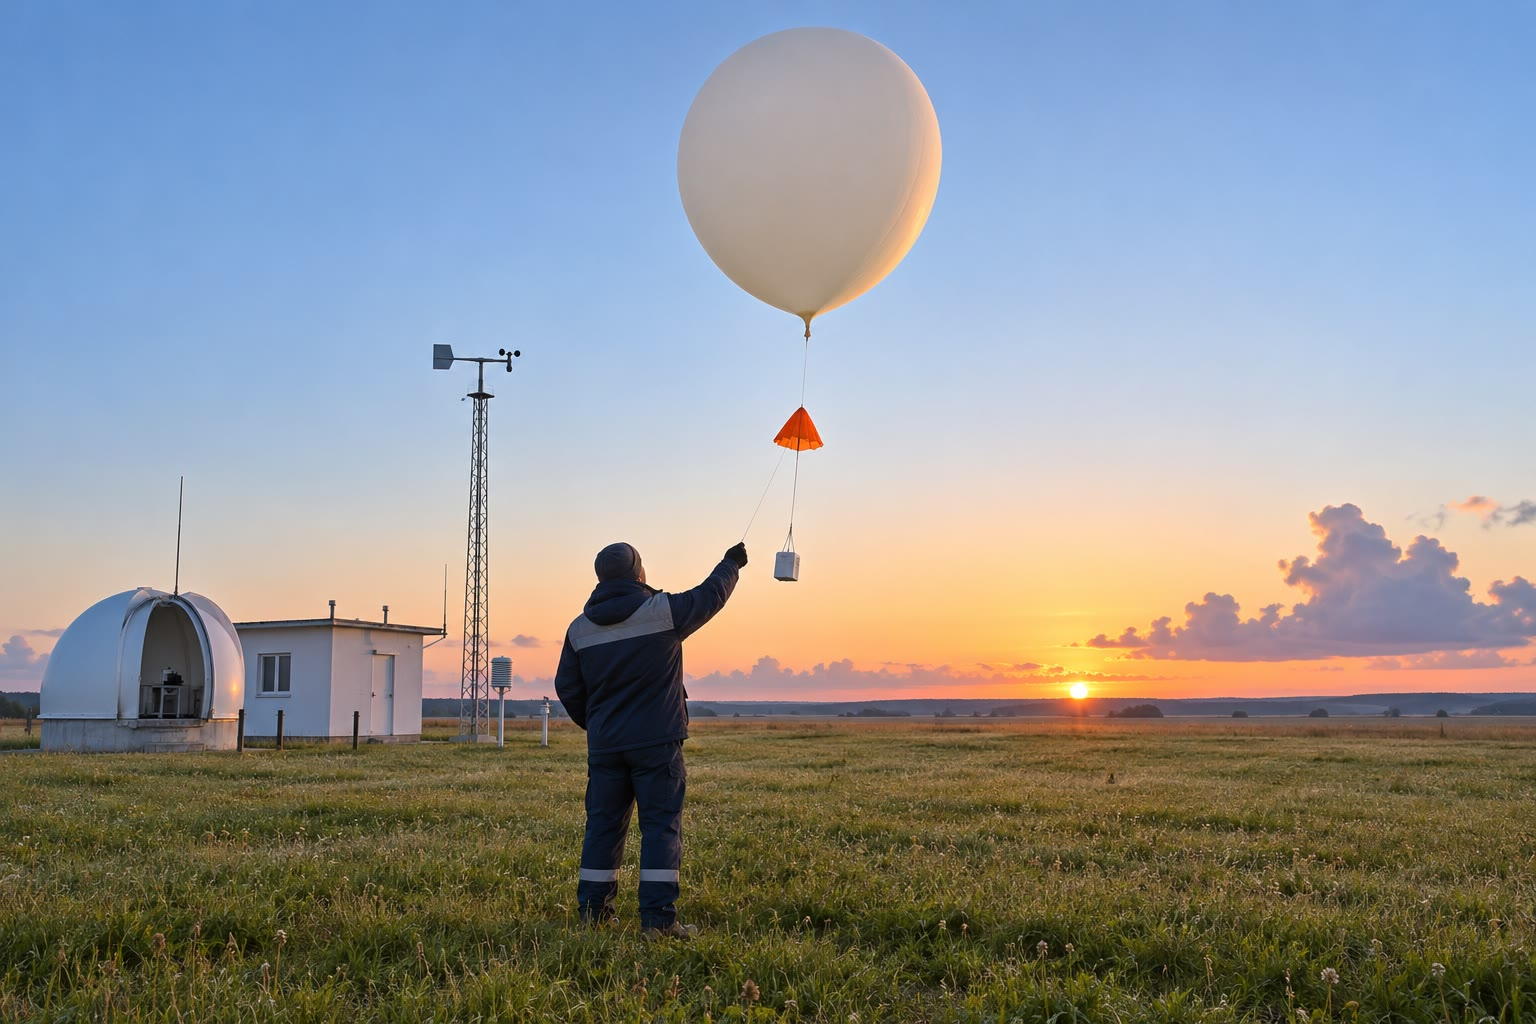
\includegraphics[width=\linewidth]{images/book4/ai/b2-radiosonde-launch.jpg}

{\scriptsize Una radiosonda lanzada al amanecer desde una estación meteorológica (ilustración
generada por IA).}
\end{minipage}
% ledger: nws:radiosonde, nws4:upperair
\end{inthefield}

\section*{Ejercicios}\label{sec:b2:atmospheric-thermodynamics:exercises}

Datos de los ejercicios, salvo aviso contrario: $e_s(T) = \qty{6.117}{hPa} \times
\exp[\qty{5419}{K} \times (1/\qty{273.16}{K} - 1/T)]$; $\varepsilon = 0.622$, $R_d =
\qty{287.0}{J.kg^{-1}.K^{-1}}$, $R_v = \qty{461.5}{J.kg^{-1}.K^{-1}}$, $c_p =
\qty{1004.5}{J.kg^{-1}.K^{-1}}$, $L = \qty{2.501e6}{J/kg}$, $g = \qty{9.81}{m.s^{-2}}$,
$\Gamma_d = \qty{9.8}{K/km}$.
% ledger: nist4:water-sat, iapws4:sublimation, const:R, earth:Mmol, nist4:water-mw, nasa:grc-gamma

\begin{exercise}[$\star$]\label{exo:b2:atmospheric-thermodynamics:1}
A \qty{850}{hPa} la temperatura es de \qty{10.0}{\celsius} y el punto de rocío de \qty{5.0}{\celsius}.
(a) Hállense la \omterm{def:b2:atmospheric-thermodynamics:moist-air}{presión de vapor} y la \omterm{def:b2:atmospheric-thermodynamics:moist-air}{presión de vapor} de saturación. (b) Hállese la humedad relativa.
(c) Hállense la \omterm{def:b2:atmospheric-thermodynamics:moist-air}{razón de mezcla} y la \omterm{def:b2:atmospheric-thermodynamics:moist-air}{humedad específica}, en gramos por kilogramo.
\end{exercise}

\begin{exercise}[$\star$]\label{exo:b2:atmospheric-thermodynamics:2}
(a) ¿En qué tanto por ciento por kelvin aumenta $e_s$ a \qty{0}{\celsius}, \qty{20}{\celsius} y
\qty{30}{\celsius}? (b) Calcúlese $e_s$ a \qty{20}{\celsius} y a \qty{25}{\celsius}, y su
cociente; compárese con $1.063^5$. (c) El valor medido a \qty{20}{\celsius} es de
\qty{23.39}{hPa}. ¿Cuánto se equivoca la fórmula, y en qué sentido? ¿Por qué?
\end{exercise}
% ledger: nist4:water-sat

\begin{exercise}[$\star$]\label{exo:b2:atmospheric-thermodynamics:3}
A mediodía el aire de superficie está a \qty{30}{\celsius} con un punto de rocío de \qty{14}{\celsius}. (a) ¿A
qué altura sobre el suelo se forman las bases de los cúmulos? (b) ¿Cuál es allí la temperatura de una porción,
según la adiabática seca? (c) ¿Cuál es allí su punto de rocío, con $\Gamma_{\text{roc}} =
\qty{1.8}{K/km}$? Coméntese. (d) Más tarde el aire se calienta hasta \qty{33}{\celsius}, con el punto de rocío
sin cambios. ¿Dónde están ahora las bases de las nubes?
\end{exercise}

\begin{exercise}[$\star$]\label{exo:b2:atmospheric-thermodynamics:4}
Léase el diagrama skew-T del sondeo de Norman. (a) ¿Hasta qué presión está saturado, o casi, el aire próximo al
suelo? (b) ¿Dónde está la inversión y cómo se manifiesta? (c) Léanse el
NCA, el NCL y el NE de la porción de superficie. (d) ¿Cómo se comparan el punto de rocío y la temperatura
justo por encima de la inversión, y qué dice eso de este aire?
\end{exercise}
% ledger: data:b4-sounding

\begin{exercise}[$\star\star$]\label{exo:b2:atmospheric-thermodynamics:5}
Un aire tropical a \qty{1000}{hPa} tiene $T = \qty{30.0}{\celsius}$ y $r = \qty{20}{g/kg}$. (a) Hállese
su \omterm{def:b2:atmospheric-thermodynamics:virtual}{temperatura virtual} de forma exacta y con la aproximación $T(1 + 0.61\,r)$. (b) Hállense las densidades
de este aire y del aire seco a la misma temperatura y presión. (c) ¿Cuánto habría que calentar el aire seco
para que fuera igual de ligero? (d) ¿Por qué importa esto para la convección sobre mares cálidos?
\end{exercise}

\begin{exercise}[$\star\star$]\label{exo:b2:atmospheric-thermodynamics:6}
Úsese la \cref{prop:b2:atmospheric-thermodynamics:gamma-s} a \qty{1000}{hPa}, con $r_s$ según la
\cref{prop:b2:atmospheric-thermodynamics:humidity}. (a) Calcúlense $r_s$ y $\Gamma_s$ a
\qty{0}{\celsius}, \qty{20}{\celsius} y \qty{30}{\celsius}. (b) ¿Cuánto más cálida que una porción seca
es una porción saturada a \qty{20}{\celsius} tras subir \qty{1}{km}, si su gradiente
no cambia? (c) ¿Por qué se reduce la diferencia más arriba?
\end{exercise}

\begin{exercise}[$\star\star$]\label{exo:b2:atmospheric-thermodynamics:7}
La porción de superficie de Norman ($p = \qty{971.1}{hPa}$, $T = \qty{19.0}{\celsius}$, $T_d =
\qty{18.5}{\celsius}$) tiene su NCA a \qty{18.35}{\celsius}. (a) Calcúlense su \omterm{def:b2:atmospheric-thermodynamics:moist-air}{razón de mezcla}, su
temperatura potencial y su \omterm{def:b2:atmospheric-thermodynamics:theta-e}{temperatura potencial equivalente}. (b) Elevada, está a
\qty{-8.9}{\celsius} a \qty{500}{hPa}, saturada. Calcúlense allí su $\theta$ y su $\theta_e$.
(c) ¿Cuál de las dos se conserva?
\end{exercise}
% ledger: data:b4-sounding

\begin{exercise}[$\star\star$]\label{exo:b2:atmospheric-thermodynamics:8}
Una porción está \qty{4}{K} más cálida que su entorno entre \qty{700}{hPa}, su NCL, y
\qty{300}{hPa}, su NE; despréciese la corrección de \omterm{def:b2:atmospheric-thermodynamics:virtual}{temperatura virtual}. (a) Calcúlese su CAPE. (b)
Calcúlese $w_{\max}$. (c) ¿En qué clase cae la CAPE? (d) En un diagrama skew-T, ¿qué
forma tiene el área positiva, y por qué su área es la calculada?
\end{exercise}
% ledger: hgx:cape

\begin{exercise}[$\star\star$]\label{exo:b2:atmospheric-thermodynamics:9}
Tómense $A = \qty{2.1}{nm}$ y el sulfato de amonio, $\kappa = 0.61$. (a) Hállense el diámetro crítico
y la \omterm{def:b2:atmospheric-thermodynamics:microphysics}{sobresaturación} crítica de una partícula seca de \qty{80}{nm}. (b) ¿Cuál es la menor partícula seca
activada en aire con una \omterm{def:b2:atmospheric-thermodynamics:microphysics}{sobresaturación} del \qty{0.3}{\percent}? ¿Y del \qty{0.1}{\percent}? (c) Una corriente ascendente
eleva la \omterm{def:b2:atmospheric-thermodynamics:microphysics}{sobresaturación} del \qty{0.1}{\percent} al \qty{0.3}{\percent}: ¿qué ocurre con el
número de gotitas, y con su tamaño para la misma agua líquida?
\end{exercise}
% ledger: pk07:kappa, pk07:kohler

\begin{exercise}[$\star\star\star$]\label{exo:b2:atmospheric-thermodynamics:10}
La porción de superficie de Norman tenía una CIN de unos \qty{-130}{J/kg} con la \omterm{def:b2:atmospheric-thermodynamics:virtual}{temperatura virtual}.
(a) ¿Con qué velocidad vertical tendría que salir del suelo para alcanzar su NCL por su propio
impulso? (b) La cima de la inversión está a \qty{889.1}{hPa} y \qty{20.5}{\celsius}. ¿Hasta qué
temperatura debe calentarse el aire de superficie a \qty{971.1}{hPa} para que una porción elevada adiabáticamente
en seco no sea más fría que la cima de la inversión? (c) Si su punto de rocío siguiera en
\qty{18.5}{\celsius}, ¿dónde estaría la base de su nube? (d) Nómbrense dos maneras en que la atmósfera
elimina una tapa así sin el sol.
\end{exercise}
% ledger: data:b4-sounding, nws4:cin

\begin{exercise}[$\star\star\star$]\label{exo:b2:atmospheric-thermodynamics:11}
(a) Demuéstrese a partir de la \cref{prop:b2:atmospheric-thermodynamics:gamma-s} que $\Gamma_s \to \Gamma_d$
cuando $r_s \to 0$. (b) Demuéstrese que cuando $Lr_s/(R_dT) \gg 1$, $\Gamma_s \to gR_vT/(LR_d)$, y
evalúese a \qty{303}{K}. (c) Compárese con el $\Gamma_{\text{roc}}$ de la
\cref{prop:b2:atmospheric-thermodynamics:lcl} cuando $T_d = T$, y explíquese por qué coinciden los dos
límites. (d) ¿Se alcanza el límite de (b) en la atmósfera? Úsese el valor $\Gamma_s =
\qty{3.4}{K/km}$ a \qty{30}{\celsius} y \qty{1000}{hPa}.
\end{exercise}

\begin{exercise}[$\star\star\star$]\label{exo:b2:atmospheric-thermodynamics:12}
Sobre el agua sobrefundida y sobre el hielo, las presiones de vapor de saturación son 2.868 y
\qty{2.599}{hPa} a \qty{-10}{\celsius}, y 1.257 y \qty{1.032}{hPa} a \qty{-20}{\celsius}.
(a) Hállese la \omterm{def:b2:atmospheric-thermodynamics:microphysics}{sobresaturación} respecto del hielo del aire saturado respecto del agua a ambas temperaturas. (b)
Compárese con las sobresaturaciones a las que se activan las gotitas. (c) Explíquese por qué una nube de
gotitas sobrefundidas que recibe unos pocos cristales de hielo se convierte en hielo. (d) ¿Por qué el efecto es
más débil cerca de \qty{0}{\celsius}?
\end{exercise}
% ledger: iapws4:sublimation, su26:svp, nws4:ccn-bergeron

\begin{problem}[{Problema de fin de semana --- Leer el sondeo de la mañana}]\label{pb:b2:atmospheric-thermodynamics:1}
La tabla da el sondeo de las 12 UTC de Norman (Oklahoma) del 16 de abril de 2026, en los niveles usados
aquí: presión, altura sobre el nivel del mar, temperatura, punto de rocío y temperatura de la
porción de superficie elevada como en el \cref{met:b2:atmospheric-thermodynamics:lift}, calculada
integrando la \cref{prop:b2:atmospheric-thermodynamics:gamma-s} a pequeños pasos. El sondeo
señala la tropopausa a \qty{235.3}{hPa} y \qty{10954}{m}. Úsense los datos de los ejercicios y
las temperaturas (no las \omterm{def:b2:atmospheric-thermodynamics:virtual}{temperaturas virtuales}) salvo indicación contraria.

\begin{center}
\small
\begin{tabular}{rrrrr}
\hline
$p$ (\unit{hPa}) & $z$ (\unit{m}) & $T$ (\unit{\celsius}) & $T_d$ (\unit{\celsius}) &
$T_{\text{porción}}$ (\unit{\celsius}) \\
\hline
971.1 & 345 & 19.0 & 18.5 & 19.0 \\
925.0 & 763 & 17.3 & 17.3 & 16.9 \\
907.7 & 924 & 16.4 & 16.4 & 16.2 \\
889.1 & 1102 & 20.5 & 9.5 & 15.4 \\
850.0 & 1489 & 18.6 & $-1.8$ & 13.7 \\
700.0 & 3110 & 4.5 & $-12.2$ & 6.1 \\
500.0 & 5725 & $-18.4$ & $-36.6$ & $-8.9$ \\
400.0 & 7357 & $-30.4$ & $-55.6$ & $-20.4$ \\
300.0 & 9349 & $-42.7$ & $-66.3$ & $-37.1$ \\
250.0 & 10560 & $-49.8$ & $-69.8$ & $-48.3$ \\
200.0 & 12006 & $-52.3$ & $-78.3$ & $-61.8$ \\
\hline
\end{tabular}
\end{center}

\medskip\noindent\textbf{Parte I --- El aire próximo al suelo.}
\begin{enumerate}
  \item Hállese la \omterm{def:b2:atmospheric-thermodynamics:moist-air}{presión de vapor} del aire de superficie, con un decimal.
  \item Hállese su \omterm{def:b2:atmospheric-thermodynamics:moist-air}{razón de mezcla}, con un decimal.
  \item Hállese su \omterm{def:b2:atmospheric-thermodynamics:moist-air}{humedad específica}.
  \item Hállese su humedad relativa.
  \item ¿Cuánto supera su \omterm{def:b2:atmospheric-thermodynamics:virtual}{temperatura virtual} a su temperatura?
  \item Hállense la altura de su NCA sobre el suelo con la regla de los \qty{125}{m}, y la presión
        allí (tómese una \omterm{def:b2:atmospheric-thermodynamics:virtual}{temperatura virtual} media de \qty{294.7}{K} para la capa).
  \item Hállese su temperatura potencial.
\end{enumerate}

\medskip\noindent\textbf{Parte II --- La tapa y las capas superiores.}
\begin{enumerate}[resume]
  \item A \qty{925}{hPa}, ¿está la porción más cálida o más fría que su entorno, y en cuánto?
  \item Hállese el gradiente entre 907.7 y \qty{889.1}{hPa}. ¿Qué clase de capa es esta?
  \item ¿En cuánto está la porción más fría que su entorno a \qty{889.1}{hPa}?
  \item Hállese la humedad relativa a \qty{850}{hPa}. ¿De dónde podría proceder un aire así?
  \item Hállese el gradiente medio entre 850 y \qty{500}{hPa} y clasifíquese la capa.
  \item Hállense el índice de levantamiento y su clase.
\end{enumerate}

\medskip\noindent\textbf{Parte III --- La energía.}
\begin{enumerate}[resume]
  \item Calcúlese el exceso $\Delta T = T_{\text{porción}} - T$ en cada nivel de la tabla.
  \item Hállese el NCL interpolando $\Delta T$ linealmente en $\ln p$, al hectopascal más próximo,
        y su altura interpolando $z$ del mismo modo.
  \item Hállense el NE y su altura del mismo modo. Compárese con la tropopausa.
  \item Calcúlese la CAPE por la regla de los trapecios en $\ln p$, desde el NCL hasta el NE pasando por los
        niveles de la tabla.
  \item ¿En qué clase cae?
  \item Calcúlese la CIN del mismo modo, desde el suelo hasta el NCL.
  \item Un cálculo sobre una malla de \qty{1}{hPa} da una CAPE de \qty{2100}{J/kg} con las
        temperaturas y de \qty{2230}{J/kg} con las \omterm{def:b2:atmospheric-thermodynamics:virtual}{temperaturas virtuales}. ¿Por qué difieren los tres
        valores?
\end{enumerate}

\medskip\noindent\textbf{Parte IV --- La tormenta que el aire podría alimentar.}
\begin{enumerate}[resume]
  \item ¿Qué velocidad vertical da la teoría de la porción con la CAPE de la pregunta 17?
  \item A la mitad de esa velocidad en todo el recorrido, ¿cuánto tardaría el aire en subir del NCL al NE?
  \item Nómbrense dos efectos que hacen más lenta una corriente ascendente real.
  \item En resumen: ¿qué velocidad de corriente ascendente predice la teoría de la porción para una tormenta alimentada por el
        aire de superficie de esta mañana?
\end{enumerate}
\end{problem}
% ledger: data:b4-sounding, hgx:cape, nws4:lifted-index, nws4:cape
